% (Zhou Junyuan) The following content is not highly relevant to the main text, so it will not be included in the body.

% In this section, we will introduce the basic data types supported by \MindQuantum. When we run quantum evolution in \MindQuantum, different data types require different sizes of computer memory and lead to different simulation accuracy.
% Before we discuss the supported data types in \MindQuantum, we first briefly review the definition of the floating-point number in modern computers which helps us understand the difference among these data types.
% The first unified technical standard of floating-point arithmetic (IEEE 754) \cite{8766229} was established in 1985 and is widely supported by various hardware today by the Institute of Electrical and Electronics Engineers (IEEE).

% In IEEE 754, a floating-point format is specified by three parts, sign, exponent, and fraction, all of which consist of a ${0,1}$ bit string as shown in Fig.~\ref{fig:ieee}.

% \begin{figure}[h]
%     \centering
%     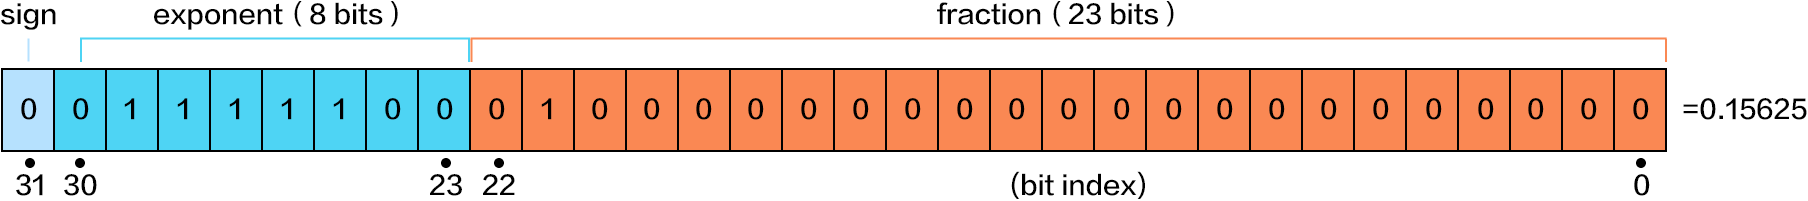
\includegraphics[width=\linewidth]{2.1_figures/Float_example.png}
%     \caption{Floating-point format}
%     \label{fig:ieee}
% \end{figure}

% The sign bit $s$ determines the sign of the number, $s=0$ is positive and $s=1$ is negative.
% The exponent part $e$ is an m-bit unsigned integer, which determines the Maximum and minimum values, and the fraction part $\vec{b}$ with $n$ bits is the true significance that appears in the memory format which determines the precision of the number.

% The real value assumed by a given sign $s$, biased exponent $e$ and fraction $\vec{b}$ as
% \begin{equation}
%     \mathrm{value} = (-1)^{s}\times 2^{e}\times (1+\sum_{i=1}^nb_{23-i}2^{-i}).
% \label[equation]{float-format}
% \end{equation}

% Based on the different numbers of bits, IEEE 754 defined three types of floating-point formats single-, double- and quadruple-precision with 32, 64, and 128 bits, respectively.
% Among them, single- and double-precision are widely used in classical computers.
% In single-precision floating-point format (for short, denoted as Single as follows), there are $1$ bit in the sign part $s$, $8$ bits in the exponent part $e$, and $23$ bits in the fraction part $\vec{b}$.
% In double-precision floating-point format (Double), there are still $1$ bit in the sign part $s$, $11$ bits in the exponent part $e$, and $52$ bits in the fraction part $\vec{b}$.

% The value precision is determined by the number of bits in the fraction part.
% In Single, the fraction part is $\vec{b}=0.b_{22}b_{21}\cdots b{0}$.
% In fact, the first $0$ is default as $1$, so the true fraction part is $1.b_{22}b_{21}\cdots b{0}$, that can explain the Eq.~\eqref{float-format} where $\vec{b}$ plus $1$.
% Then the total precision of Single is 24 bits which approximates $7.22$ decimal digits as $\log_{10}(2^{24}) \approx 7.225$.
% As similar, the total precision of Double is $53$ which can approximate $\log_{10}(2^{53}) \approx 15.95$ decimal digits.
% There is an interesting example showing the difference in the precision of Single and Double,
% \begin{lstlisting}
% z_32=0.1f0+0.2f0
% print(z_32)
% 0.30000001192092896
% z_64=0.1+0.2
% print(z_64)
% 0.30000000000000004
% \end{lstlisting}
% which shows that Single can get $7$ significant digits and Double get $16$ significant digits.


在量子计算中，复数是刻画量子信息的基本工具。复数属于一种在实数基础上引入特定元素 $i$ 后得到的数系，其中 $i$ 称为虚数单位，并满足方程 $i^2=-1$。
复数可以表示为 $c=a+bi$ 的形式，其中 $a$ 和 $b$ 均为实数，$a$ 称为实部，$b$ 称为虚部。

在计算机数字格式中，复数 $c$ 的数据类型由 $a$ 和 $b$ 的类型决定。
通常，如果 $a$ 和 $b$ 均为单精度（Single），则 $c$ 的类型为 complex64（使用 64 位存储 $c$）；如果 $a$ 和 $b$ 均为双精度（Double），则 $c$ 的类型为 complex128（使用 128 位存储 $c$）。

在不同编程语言中，虚数单位的符号可能有所不同。
例如，在 C 语言中，$i$ 表示为 $I$；在 Python 中，则表示为 $1j$。
\MindQuantum\ 支持单精度和双精度浮点格式，同时也支持它们对应的复数格式；这些复数格式对于模拟量子演化不可或缺。
这些数据类型可以与 NumPy \cite{harris2020array} 包中的对应数据类型便捷转换。它们具有相同的数学性质，但在 \MindQuantum\ 中使用时，相比直接声明为 NumPy 数据类型更便于框架内部处理。

\begin{lstlisting}
import numpy as np
import mindquantum as mq

# 支持不同类型
all_types = [mq.float32, mq.float64, mq.complex64, mq.complex128]

# 与 numpy 类型相互转换
mq_float64 = mq.to_mq_type(np.float64)
numpy_float64 = mq.to_np_type(mq.float64)
\end{lstlisting}

指数墙是在经典计算机上模拟量子系统面临的主要障碍。
随着量子系统规模增大，所需经典资源会呈指数增长。
一个包含 $N$ 个量子比特的量子态可以由 $2^N$ 个振幅描述，而所有振幅都是复数。

如果要存储一个 $N=20$ 的量子态，其中包含 $2^{20}$ 个振幅，且所有振幅均以单精度（Complex64）表示，则所需经典内存为
\begin{equation}
    G=2^{20}\times 64 \mathrm{bits} = 8 \mathrm{MB}.
\end{equation}

如果使用双精度复数表示振幅，则内存需求为 $G=2^{20}\times 128 \mathrm{bits}=16 \mathrm{MB}$。下面的表格展示了在不同数据精度下存储全振幅量子态所需的内存消耗。

\begin{table}[ht]
    \begin{tabular}{ccc}
        \toprule
        量子比特数 & Complex128 & Complex64 \\
        \midrule
        6            & 1kB        & 0.5kB     \\
        16           & 1MB        & 0.5MB     \\
        26           & 1GB        & 0.5GB     \\
        30           & 16GB       & 8GB       \\
        36           & 1TB        & 0.5TB     \\
        40           & 16TB       & 8TB       \\
        \bottomrule
    \end{tabular}
    \caption{存储全振幅量子态的内存消耗。}
    \label{tab:mem_consume}
\end{table}

不难看出，双精度所需存储空间是单精度的两倍，因为每个双精度振幅占用 $128$ 位，而每个单精度振幅占用 $64$ 位。
虽然双精度需要更多空间，通常也需要更多计算时间（这取决于具体处理单元），但它能够提供更高精度；这对于量子计算中的一些任务非常重要，例如求解量子哈密顿量的本征值。
事实上，在相同内存资源下，使用单精度表示振幅相比双精度最多只能多模拟一个量子比特。
因此，如果内存资源充足，我们强烈建议优先使用双精度复数。
